\section{Introduction}
\labsec{intro}

Ever since the sequence of the human genome was made available some 20 
years ago, \sidecite[-1\baselineskip]{Lander2001a} one of the most 
compelling goals in both science and medicine has been that of finding 
the genetic variants associated to diseases.

% The first attempts relied on statistical association tests, like the 
% $\chi^2$ test, to identify the genetic variants that are more likely to 
% occur in ill rather than healthy individuals. \sidecite{Visscher2012a} 
% Despite its successes, the power of this approach is hampered by the 
% fact that there are so many genetic variants (on average, the DNA 
% sequences of two non-related people differ of about one letter every one 
% thousand \sidecite{Durbin2010}), most of which, the so-called rare 
% variants, appear only in a tiny fraction of individuals.

In 2015 it was proposed a new method, 
\sidecite[-1.1cm]{Gamazon2015a} dubbed Transcriptome-Wide 
Association Study (TWAS), which consists of using the genetic variants 
to predict gene expression, and then finding associations between the 
predicted expression and a disease. The first advantage is that it is 
possible to avoid a direct measurement of gene expression, which can be 
expensive or even impossible for certain tissues. But another, more 
subtle advantage is that predicted values are less noisy than the real 
ones, because they do not include the environmental component of 
expression (\refeq{expr}). In view of this method, predicting gene 
expression is a relevant problem.

A gene is a region of DNA, and its expression can be defined as the 
amount of RNA molecules that originate from that region 
(\vreffig{response}). This amount is different in different individuals, 
and our goal is to predict these differences.

\begin{marginfigure}[-3.8cm]
  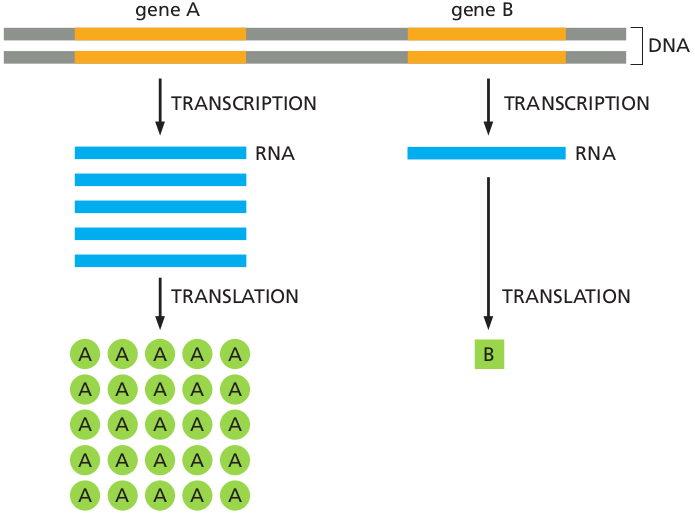
\includegraphics{response}
  \caption{Each gene is \enquote{transcribed} into many RNA molecules, 
which then are \enquote{translated} into proteins.}
  \labfig{response}
\end{marginfigure}

As regards the DNA itself, in this context it can be regarded as a 
3-billion letter long string, different for each individual. Most of the 
postions in the sequence are the same, but there are some specific 
positions, called polymorphic loci, which harbour different letters in 
different people (\reffig{predictorsA}). There are many kinds of 
differences, but, as similar works do, 
\sidecite[-8.6cm]{Nagpal2019} here we will focus only on 
single-letter differences such that in the population only two letters 
are present, \ie we will only consider those positions that can be in 
two states.

\begin{marginfigure}[-1.5cm]
\setlength{\tabcolsep}{2pt}
\scalebox{0.7}{%
\begin{subfigure}{\textwidth}
  \caption{}
  \labfig{predictorsA}
  \small
  \texttt{%
  \begin{tabular}{l c c c c c c c c c c c c c c c c c c}
	\textsf{Alice\hspace{.2cm}} & A & T & G & \cellcolor{yellow}G	& T & G & \cellcolor{cyan}C		& T & G & T & C & T & C & C & T & G & \cellcolor{red}T	& C \\
	\textsf{Bob\hspace{.2cm}}   & A & T & G & \cellcolor{yellow}G	& T & G & \cellcolor{cyan}C		& T & G & T & C & T & C & C & T & G & \cellcolor{cyan}C	& C \\
	\textsf{Craig\hspace{.2cm}} & A & T & G & \cellcolor{green}A	& T & G & \cellcolor{green}A	& T & G & T & C & T & C & C & T & G & \cellcolor{cyan}C	& C \\
	\textsf{Dave\hspace{.2cm}}  & A & T & G & \cellcolor{green}A	& T & G & \cellcolor{cyan}C		& T & G & T & C & T & C & C & T & G & \cellcolor{cyan}C	& C \\
	\textsf{Eve\hspace{.2cm}}   & A & T & G & \cellcolor{yellow}G	& T & G & \cellcolor{green}A	& T & G & T & C & T & C & C & T & G & \cellcolor{red}T	& C \\
	\textsf{Frank\hspace{.2cm}} & A & T & G & \cellcolor{yellow}G	& T & G & \cellcolor{green}A	& T & G & T & C & T & C & C & T & G & \cellcolor{cyan}C	& C \\
  \end{tabular}}
\end{subfigure}
}

\scalebox{0.7}{%
\begin{subfigure}{\textwidth}
  \caption{}
  \labfig{predictorsB}
  \small
  \texttt{%
  \begin{tabular}{l c c c c c c c c c c c c c c c c c c}
	\textsf{Alice\hspace{.2cm}} & \phantom{A} & \phantom{A} & \phantom{A} & 0 & \phantom{A} & \phantom{A} & 0 & \phantom{A} & \phantom{A} & \phantom{A} & \phantom{A} & \phantom{A} & \phantom{A} & \phantom{A} & \phantom{A} & \phantom{A} & 1 & \phantom{A} \\
	\textsf{Bob\hspace{.2cm}}   & \phantom{A} & \phantom{A} & \phantom{A} & 0 & \phantom{A} & \phantom{A} & 0 & \phantom{A} & \phantom{A} & \phantom{A} & \phantom{A} & \phantom{A} & \phantom{A} & \phantom{A} & \phantom{A} & \phantom{A} & 0 & \phantom{A} \\
	\textsf{Craig\hspace{.2cm}} & \phantom{A} & \phantom{A} & \phantom{A} & 1 & \phantom{A} & \phantom{A} & 1 & \phantom{A} & \phantom{A} & \phantom{A} & \phantom{A} & \phantom{A} & \phantom{A} & \phantom{A} & \phantom{A} & \phantom{A} & 0 & \phantom{A} \\
	\textsf{Dave\hspace{.2cm}}  & \phantom{A} & \phantom{A} & \phantom{A} & 1 & \phantom{A} & \phantom{A} & 0 & \phantom{A} & \phantom{A} & \phantom{A} & \phantom{A} & \phantom{A} & \phantom{A} & \phantom{A} & \phantom{A} & \phantom{A} & 0 & \phantom{A} \\
	\textsf{Eve\hspace{.2cm}}   & \phantom{A} & \phantom{A} & \phantom{A} & 0 & \phantom{A} & \phantom{A} & 1 & \phantom{A} & \phantom{A} & \phantom{A} & \phantom{A} & \phantom{A} & \phantom{A} & \phantom{A} & \phantom{A} & \phantom{A} & 1 & \phantom{A} \\
	\textsf{Frank\hspace{.2cm}} & \phantom{A} & \phantom{A} & \phantom{A} & 0 & \phantom{A} & \phantom{A} & 1 & \phantom{A} & \phantom{A} & \phantom{A} & \phantom{A} & \phantom{A} & \phantom{A} & \phantom{A} & \phantom{A} & \phantom{A} & 0 & \phantom{A} \\
  \end{tabular}}
\end{subfigure}
}
\caption{(a) Examples of DNA sequences; polymorphic loci are highligthed 
with different colours. (b) Predictors matrix built from the sequences 
in (a).}
\labfig{predictors}
\end{marginfigure}

DNA lends itself to a representation where the positions that are the 
same in all the individuals are ignored, and the two possible letters of 
these polymorphic loci are encoded as zeroes or ones 
(\reffig{predictorsB}). Indeed, all the published works on this topic 
use a matrix of this kind, constructed on a window of one million 
letters around each gene. Moreover, each gene is treated independently 
of all the others, and one model is run for each gene. The expression of 
gene $A$ in individual $i$ can be modeled as in \vrefeq{expr}, where 
$X_{ij}$ is the genotype (0 or 1) of individual $i$ at locus $j$, and 
$\beta_j$ is the increase in expression for individuals that have a 1 at 
locus $j$ with respect to the other individuals. Importantly, this is an 
additive model and no interactions are considered.

%\marginnote[-1.3cm]
